\documentclass{standalone}
\usepackage{tikz}
\usetikzlibrary{patterns}
\usetikzlibrary{positioning}
\usetikzlibrary{patterns, positioning}
\usetikzlibrary{shapes.misc}
\usepackage[outline]{contour}
\contourlength{1.5pt} 
\usepackage[sfdefault]{ClearSans}

\begin{document}
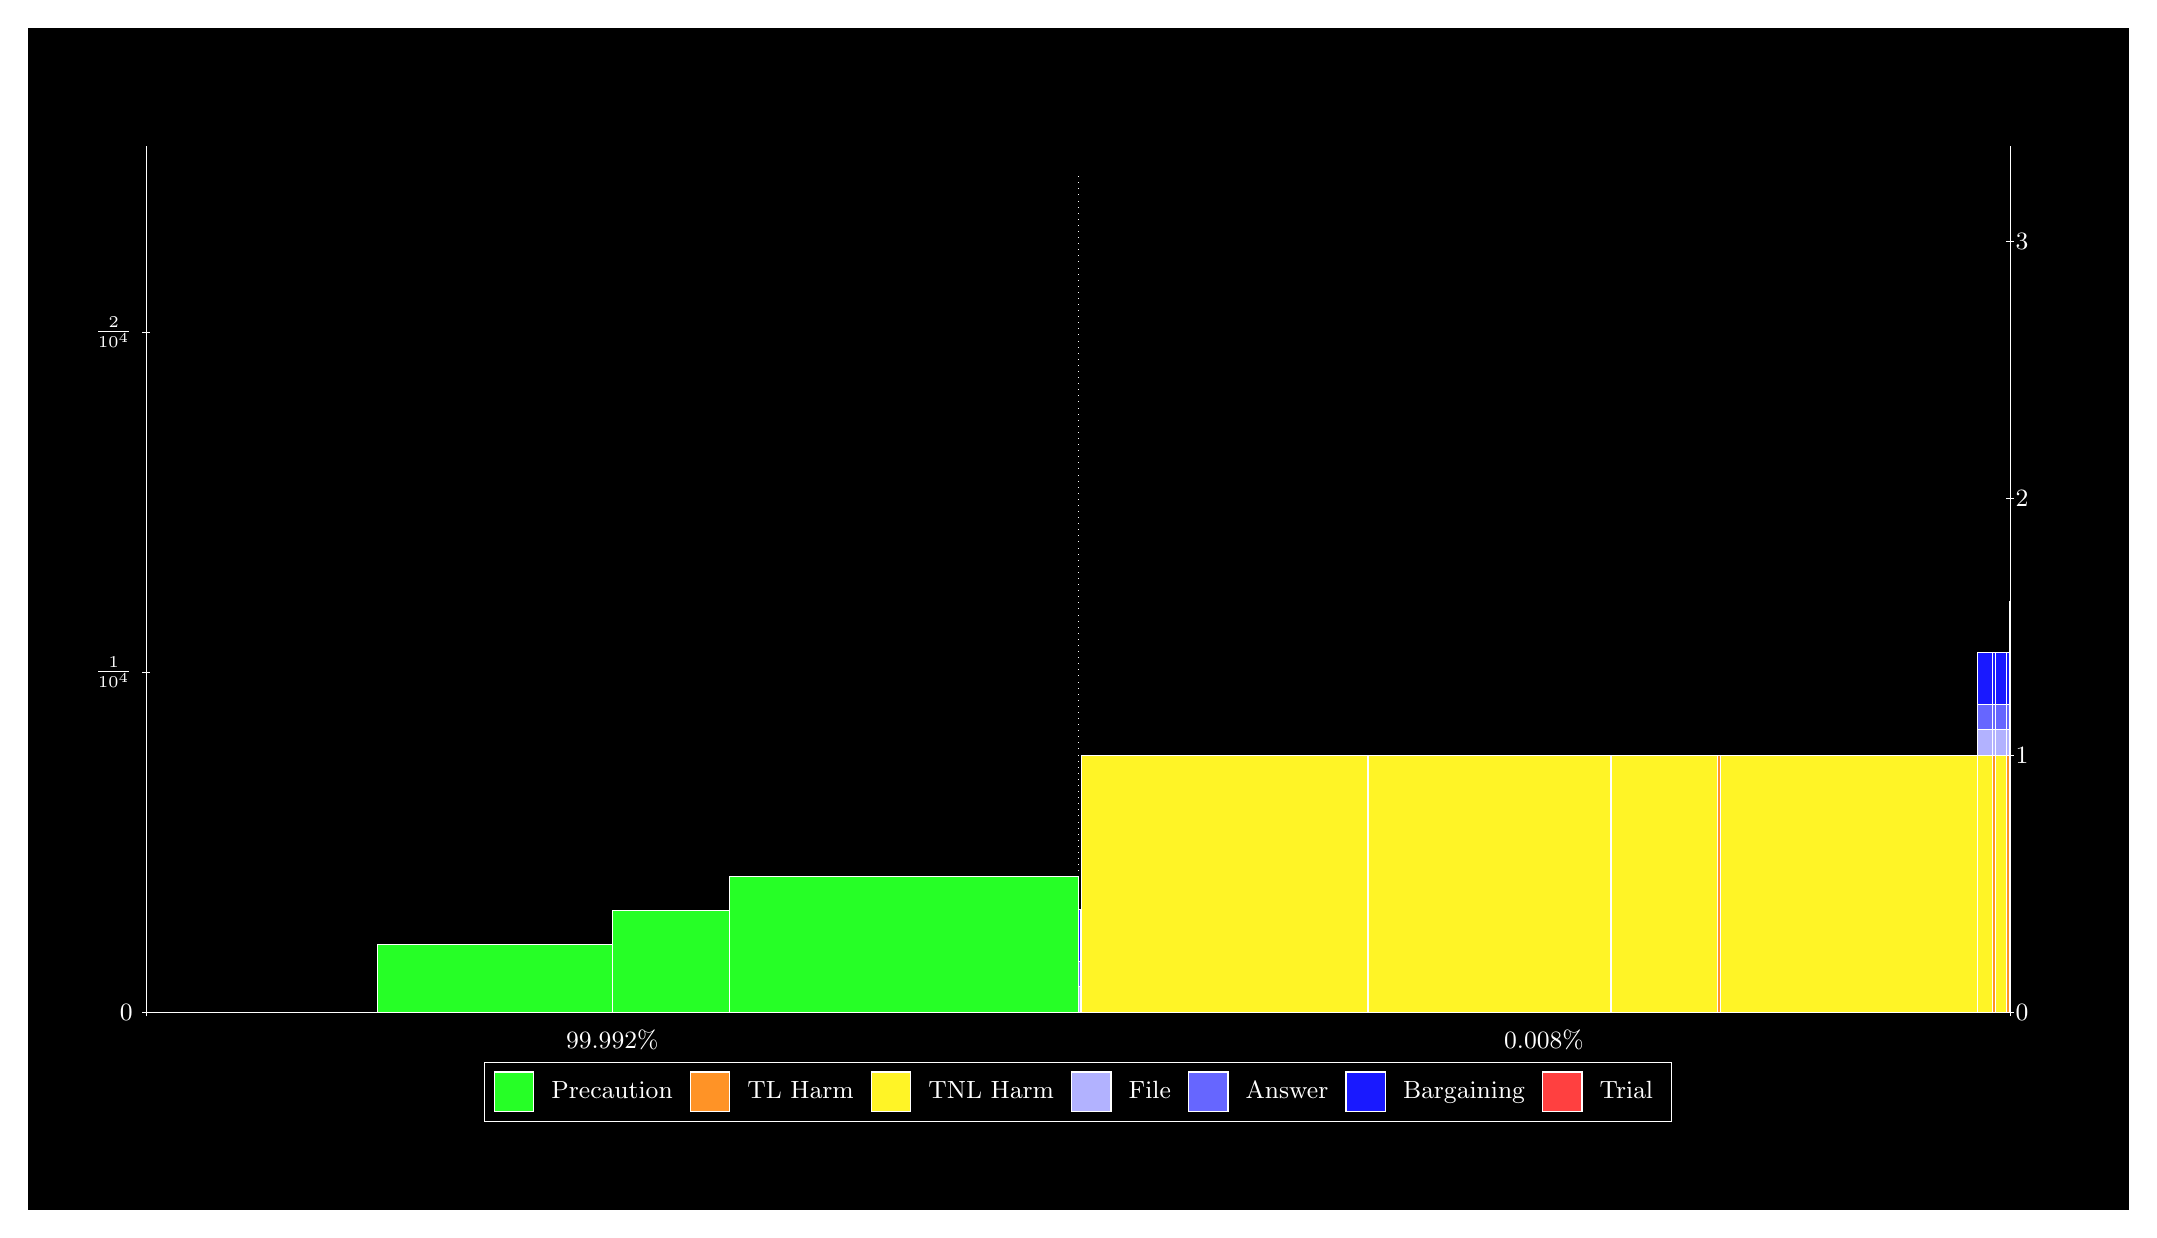
\begin{tikzpicture}
\draw[fill=black] (0,0) rectangle (26.667,15);
\draw[fill=green!85,draw=white,very thin] (4.43,2.5) rectangle (7.4166,3.3641);
\draw[fill=green!85,draw=white,very thin] (7.4166,2.5) rectangle (8.898,3.7962);
\draw[fill=green!85,draw=white,very thin] (8.898,2.5) rectangle (13.333,4.2282);
\draw[fill=blue!30,draw=white,very thin] (13.333,2.5) rectangle (13.356,2.8266);
\draw[fill=blue!60,draw=white,very thin] (13.333,2.8266) rectangle (13.356,3.1531);
\draw[fill=blue!90,draw=white,very thin] (13.333,3.1531) rectangle (13.356,3.8062);
\draw[fill=green!85,draw=white,very thin] (13.356,2.5) rectangle (13.378,2.5001);
\draw[fill=blue!30,draw=white,very thin] (13.356,2.5001) rectangle (13.378,2.8266);
\draw[fill=blue!60,draw=white,very thin] (13.356,2.8266) rectangle (13.378,3.1532);
\draw[fill=blue!90,draw=white,very thin] (13.356,3.1532) rectangle (13.378,3.8063);
\draw[fill=yellow!85,draw=white,very thin] (13.378,2.5) rectangle (17.012,5.7656);
\draw[fill=orange!85,draw=white,very thin] (17.012,2.5) rectangle (17.024,5.7656);
\draw[fill=green!85,draw=white,very thin] (17.024,2.5) rectangle (20.097,2.5001);
\draw[fill=yellow!85,draw=white,very thin] (17.024,2.5001) rectangle (20.097,5.7657);
\draw[fill=green!85,draw=white,very thin] (20.097,2.5) rectangle (20.107,2.5001);
\draw[fill=orange!85,draw=white,very thin] (20.097,2.5001) rectangle (20.107,5.7657);
\draw[fill=green!85,draw=white,very thin] (20.107,2.5) rectangle (21.449,2.5001);
\draw[fill=yellow!85,draw=white,very thin] (20.107,2.5001) rectangle (21.449,5.7657);
\draw[fill=green!85,draw=white,very thin] (21.449,2.5) rectangle (21.488,2.5001);
\draw[fill=orange!85,draw=white,very thin] (21.449,2.5001) rectangle (21.488,5.7657);
\draw[fill=green!85,draw=white,very thin] (21.488,2.5) rectangle (24.757,2.5001);
\draw[fill=yellow!85,draw=white,very thin] (21.488,2.5001) rectangle (24.757,5.7657);
\draw[fill=yellow!85,draw=white,very thin] (24.757,2.5) rectangle (24.941,5.7656);
\draw[fill=blue!30,draw=white,very thin] (24.757,5.7656) rectangle (24.941,6.0922);
\draw[fill=blue!60,draw=white,very thin] (24.757,6.0922) rectangle (24.941,6.4187);
\draw[fill=blue!90,draw=white,very thin] (24.757,6.4187) rectangle (24.941,7.0719);
\draw[fill=orange!85,draw=white,very thin] (24.941,2.5) rectangle (24.982,5.7656);
\draw[fill=blue!30,draw=white,very thin] (24.941,5.7656) rectangle (24.982,6.0922);
\draw[fill=blue!60,draw=white,very thin] (24.941,6.0922) rectangle (24.982,6.4187);
\draw[fill=blue!90,draw=white,very thin] (24.941,6.4187) rectangle (24.982,7.0719);
\draw[fill=green!85,draw=white,very thin] (24.982,2.5) rectangle (25.125,2.5001);
\draw[fill=yellow!85,draw=white,very thin] (24.982,2.5001) rectangle (25.125,5.7657);
\draw[fill=blue!30,draw=white,very thin] (24.982,5.7657) rectangle (25.125,6.0922);
\draw[fill=blue!60,draw=white,very thin] (24.982,6.0922) rectangle (25.125,6.4188);
\draw[fill=blue!90,draw=white,very thin] (24.982,6.4188) rectangle (25.125,7.0719);
\draw[fill=green!85,draw=white,very thin] (25.125,2.5) rectangle (25.157,2.5001);
\draw[fill=orange!85,draw=white,very thin] (25.125,2.5001) rectangle (25.157,5.7657);
\draw[fill=blue!30,draw=white,very thin] (25.125,5.7657) rectangle (25.157,6.0922);
\draw[fill=blue!60,draw=white,very thin] (25.125,6.0922) rectangle (25.157,6.4188);
\draw[fill=blue!90,draw=white,very thin] (25.125,6.4188) rectangle (25.157,7.0719);
\draw[fill=yellow!85,draw=white,very thin] (25.157,2.5) rectangle (25.16,5.7656);
\draw[fill=blue!30,draw=white,very thin] (25.157,5.7656) rectangle (25.16,6.0922);
\draw[fill=blue!60,draw=white,very thin] (25.157,6.0922) rectangle (25.16,6.4187);
\draw[fill=blue!90,draw=white,very thin] (25.157,6.4187) rectangle (25.16,7.0719);
\draw[fill=red!75,draw=white,very thin] (25.157,7.0719) rectangle (25.16,7.725);
\draw[fill=orange!85,draw=white,very thin] (25.16,2.5) rectangle (25.163,5.7656);
\draw[fill=blue!30,draw=white,very thin] (25.16,5.7656) rectangle (25.163,6.0922);
\draw[fill=blue!60,draw=white,very thin] (25.16,6.0922) rectangle (25.163,6.4187);
\draw[fill=blue!90,draw=white,very thin] (25.16,6.4187) rectangle (25.163,7.0719);
\draw[fill=red!75,draw=white,very thin] (25.16,7.0719) rectangle (25.163,7.725);
\draw[fill=green!85,draw=white,very thin] (25.163,2.5) rectangle (25.165,2.5001);
\draw[fill=yellow!85,draw=white,very thin] (25.163,2.5001) rectangle (25.165,5.7657);
\draw[fill=blue!30,draw=white,very thin] (25.163,5.7657) rectangle (25.165,6.0922);
\draw[fill=blue!60,draw=white,very thin] (25.163,6.0922) rectangle (25.165,6.4188);
\draw[fill=blue!90,draw=white,very thin] (25.163,6.4188) rectangle (25.165,7.0719);
\draw[fill=red!75,draw=white,very thin] (25.163,7.0719) rectangle (25.165,7.7251);
\draw[fill=green!85,draw=white,very thin] (25.165,2.5) rectangle (25.167,2.5001);
\draw[fill=orange!85,draw=white,very thin] (25.165,2.5001) rectangle (25.167,5.7657);
\draw[fill=blue!30,draw=white,very thin] (25.165,5.7657) rectangle (25.167,6.0922);
\draw[fill=blue!60,draw=white,very thin] (25.165,6.0922) rectangle (25.167,6.4188);
\draw[fill=blue!90,draw=white,very thin] (25.165,6.4188) rectangle (25.167,7.0719);
\draw[fill=red!75,draw=white,very thin] (25.165,7.0719) rectangle (25.167,7.7251);
\draw[white,very thin] (1.5,2.5) -- (1.5,13.5);
\draw[white,very thin] (1.45,2.5) -- (1.55,2.5);
\node[font=\small,text=white, anchor=east] at (1.45, 2.5) {0};
\draw[white,very thin] (1.45,6.8206) -- (1.55,6.8206);
\node[font=\small,text=white, anchor=east] at (1.45, 6.8206) {$\frac{1}{10^{4}}$};
\draw[white,very thin] (1.45,11.141) -- (1.55,11.141);
\node[font=\small,text=white, anchor=east] at (1.45, 11.141) {$\frac{2}{10^{4}}$};

\draw[white,dotted,very thin] (13.333,2.83) -- (13.333,13.17);
\draw[white,very thin] (25.167,2.5) -- (25.167,13.5);
\draw[white,very thin] (25.117,2.5) -- (25.217,2.5);
\node[font=\small,text=white, anchor=west] at (25.117, 2.5) {0};
\draw[white,very thin] (25.117,5.7656) -- (25.217,5.7656);
\node[font=\small,text=white, anchor=west] at (25.117, 5.7656) {1};
\draw[white,very thin] (25.117,9.0312) -- (25.217,9.0312);
\node[font=\small,text=white, anchor=west] at (25.117, 9.0312) {2};
\draw[white,very thin] (25.117,12.297) -- (25.217,12.297);
\node[font=\small,text=white, anchor=west] at (25.117, 12.297) {3};

\draw[white,very thin] (1.5,2.5) -- (25.167,2.5);
\draw[white,very thin] (1.5,2.45) -- (1.5,2.55);
\node[font=\small,text=white, anchor=north] at (1.5, 2.45) {};
\draw[white,very thin] (25.167,2.45) -- (25.167,2.55);
\node[font=\small,text=white, anchor=north] at (25.167, 2.45) {};

\node[font=\small,text=white,anchor=south] at (7.4167, 1.9) {99.992\%};
\node[font=\small,text=white,anchor=south] at (19.25, 1.9) {0.008\%};
\draw (13.3333,2.5) node (B) {};
\begin{scope}[align=center]
\matrix[scale=0.5,draw=white,below=0.5cm of B,nodes={draw},column sep=0.1cm]{
\node[rectangle,draw,minimum width=0.5cm,minimum height=0.5cm,fill=green!85]{}; & \node[draw=none,font=\small,text=white]{Precaution}; &
\node[rectangle,draw,minimum width=0.5cm,minimum height=0.5cm,fill=orange!85]{}; & \node[draw=none,font=\small,text=white]{TL Harm}; &
\node[rectangle,draw,minimum width=0.5cm,minimum height=0.5cm,fill=yellow!85]{}; & \node[draw=none,font=\small,text=white]{TNL Harm}; &
\node[rectangle,draw,minimum width=0.5cm,minimum height=0.5cm,fill=blue!30]{}; & \node[draw=none,font=\small,text=white]{File}; &
\node[rectangle,draw,minimum width=0.5cm,minimum height=0.5cm,fill=blue!60]{}; & \node[draw=none,font=\small,text=white]{Answer}; &
\node[rectangle,draw,minimum width=0.5cm,minimum height=0.5cm,fill=blue!90]{}; & \node[draw=none,font=\small,text=white]{Bargaining}; &
\node[rectangle,draw,minimum width=0.5cm,minimum height=0.5cm,fill=red!75]{}; & \node[draw=none,font=\small,text=white]{Trial}; \\\\
};\end{scope}

\end{tikzpicture}
\end{document}